\documentclass{article}
\usepackage{amsmath}
\usepackage{amssymb}
\usepackage{graphicx}
\usepackage{hyperref}
\usepackage[version=4]{mhchem}

\title{Example 19}
\date{}

\begin{document}
\maketitle

(2002 AIME II) In triangle \(A B C\), point \(D\) is on \(B C\) with \(C D=2\) and \(D B=5\), point \(E\) is on \(A C\) with \(C E=1\) and \(E A=3, A B=8\), and \(A D\) and \(B E\) intersect at \(P\). Points \(Q\) and \(R\) lie on \(A B\) so that \(P Q\) is parallel to \(C A\) and \(P R\) is parallel to \(C B\). It is given that the ratio of the area of triangle \(P Q R\) to the area\\
\centering
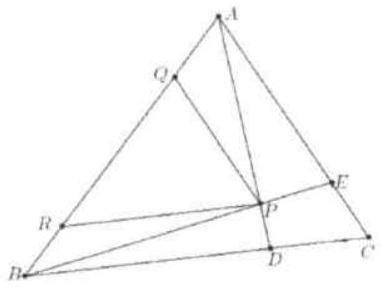
\includegraphics[width=\textwidth]{images/121(2).jpg}\\
of triangle \(A B C\) is \(m / n\), where \(m\) and \(n\) are relatively prime positive integers. Find \(m+n\).

Solution: 901.\\
Method 1 (official solution):\\
Draw the line through \(E\) parallel to \(A D\), and let \(K\) be its intersection with \(B C\).\\
Because \(C D=2\) and \(K C: K D=E C: E A=1: 3\), it follows that \(K D=3 / 2\).\\
\centering
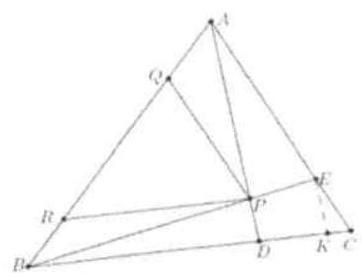
\includegraphics[width=\textwidth]{images/122.jpg}

Therefore, \(\frac{Q P}{A E}=\frac{B P}{B E}=\frac{B D}{B K}=\frac{5}{5+\frac{3}{2}}=\frac{10}{13}\). Thus\\
\(\frac{Q P}{A C}=\frac{3}{4} \cdot \frac{10}{13}=\frac{15}{26}\).\\
Since triangles \(P Q R\) and \(C A B\) are similar, the ratio of their areas is \((15 / 26)^{2}=\) \(225 / 676\). Thus \(m+n=901\).

Method 2 (our solution):\\
Draw the line through \(D\) parallel to \(B E\), and let \(F\) be its intersection with \(A C\).

Observe that triangles \(B E C\) and \(D F C\) are similar.\\
\(\frac{B C}{D C}=\frac{E C}{F C} \quad \Rightarrow \quad \frac{7}{2}=\frac{1}{F C} \quad \Rightarrow \quad F C=\frac{2}{7}\)\\
\centering
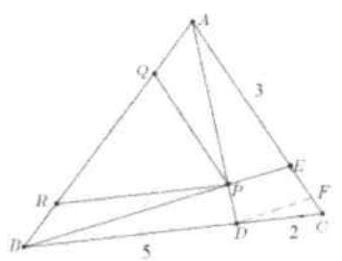
\includegraphics[width=\textwidth]{images/122(1).jpg}

So \(E F=\frac{5}{7}\).\\
Triangles \(R P A\) and \(B D A\) are similar.\\
It follows that \(\frac{R P}{B D}=\frac{A P}{A D}\).\\
Since triangles \(A D F\) and \(A P E\) are similar, so \(\frac{A E}{A F}=\frac{A P}{A D}\).\\
\centering
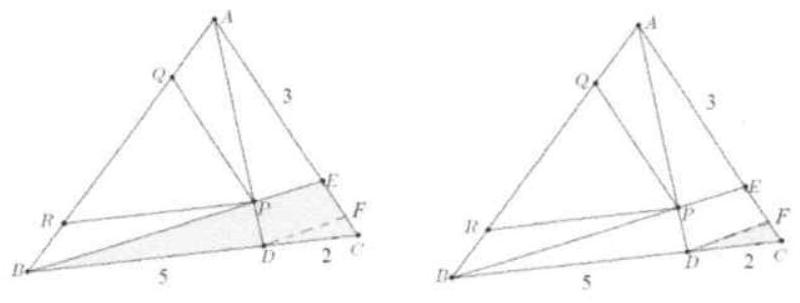
\includegraphics[width=\textwidth]{images/122(2).jpg}


Thus, \(\frac{R P}{B D}=\frac{A P}{A D}=\frac{A E}{A F}=\frac{3}{3+\frac{5}{7}}=\frac{21}{26} \Rightarrow R P=\frac{21}{26} \times 5\).\\
Since triangles \(P Q R\) and \(C A B\) are similar, the ratio of their areas is\\
\(\frac{S_{\triangle P Q R}}{S_{\triangle A B C}}=\left(\frac{R P}{B C}\right)^{2}=\left(\frac{\frac{21}{26} \times 5}{7}\right)^{2}=\left(\frac{15}{26}\right)^{2}=\frac{225}{676}\)\\
Thus \(m+n=901\).\\
This is the problem 13 in 2002 AIME II.\\
\centering
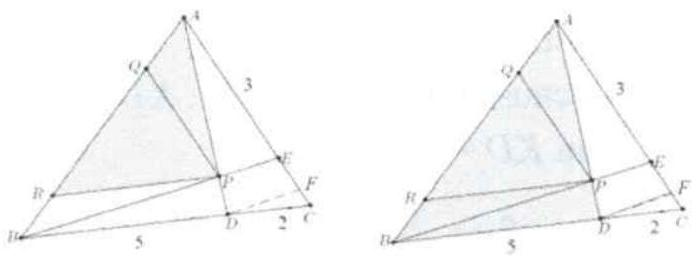
\includegraphics[width=\textwidth]{images/123(2).jpg}


\end{document}
